\chapter{Analysing GDPR Compliance Requirements}
\label{chapter:information}

This chapter presents an analysis of information about activities associated with personal data and consent towards generating requirements for GDPR compliance. \autoref{sec:info:model} presents an analysis of GDPR in terms of stakeholders and interoperability of information between them along with an analysis of suitability of existing standards to represent it. Following this, \autoref{sec:info:compliance-questions} frames `compliance questions' that provide information requirements necessary to evaluate compliance. \autoref{sec:info:competency-questions} uses the compliance questions and identified gaps within the state of the art to formulate competency questions towards developing necessary ontologies for information representation of GDPR and activities involving personal data and consent. Finally, \autoref{sec:info:constraints} presents the assumptions and constraints over information that can be used to validate the information for correctness and completeness.

\section{Interoperability Model of Information based on GDPR}\label{sec:info:model}

This section presents an analyses of the GDPR in terms of information requirements of stakeholders and presents a model of interoperability between them. The model enables understanding the role of stakeholders in the compliance process and provides a framework to analyse approaches in the state of the art to meet requirements. The model also provides motivation to incorporate interoperability as a core requirement within representations of information towards GDPR compliance.
The work described in this section was published in a conference paper
\cite{pandit_gdpr_2018} which was later expanded upon in a journal article \cite{pandit_exploration_2018}. % EURAS, IJSR

The entity in terms of GDPR compliance are as follows: Data Subject (DS), Data Controller (DC), Data Processor (DP) and Supervisory Authority\footnote{Supervisory Authority are also referred to as Data Protection Commission or Regulatory Body} (SA). In addition to this, if a controller or processor uses a Data Management (DM) interface or service for their compliance operations, it can be a considered as a separate entity given its autonomous operations and possible provision by a third party. Though the GDPR does not mention or allude to the functionality of DM, it is included as a virtual entity in the analyses for practical reasons as a point of interoperability between entities.

With this, there are 11 possible points of interactions between entities, as summarised in Figure \ref{fig:info:interoperability-model}.
\begin{figure}[htbp]
    \centering
    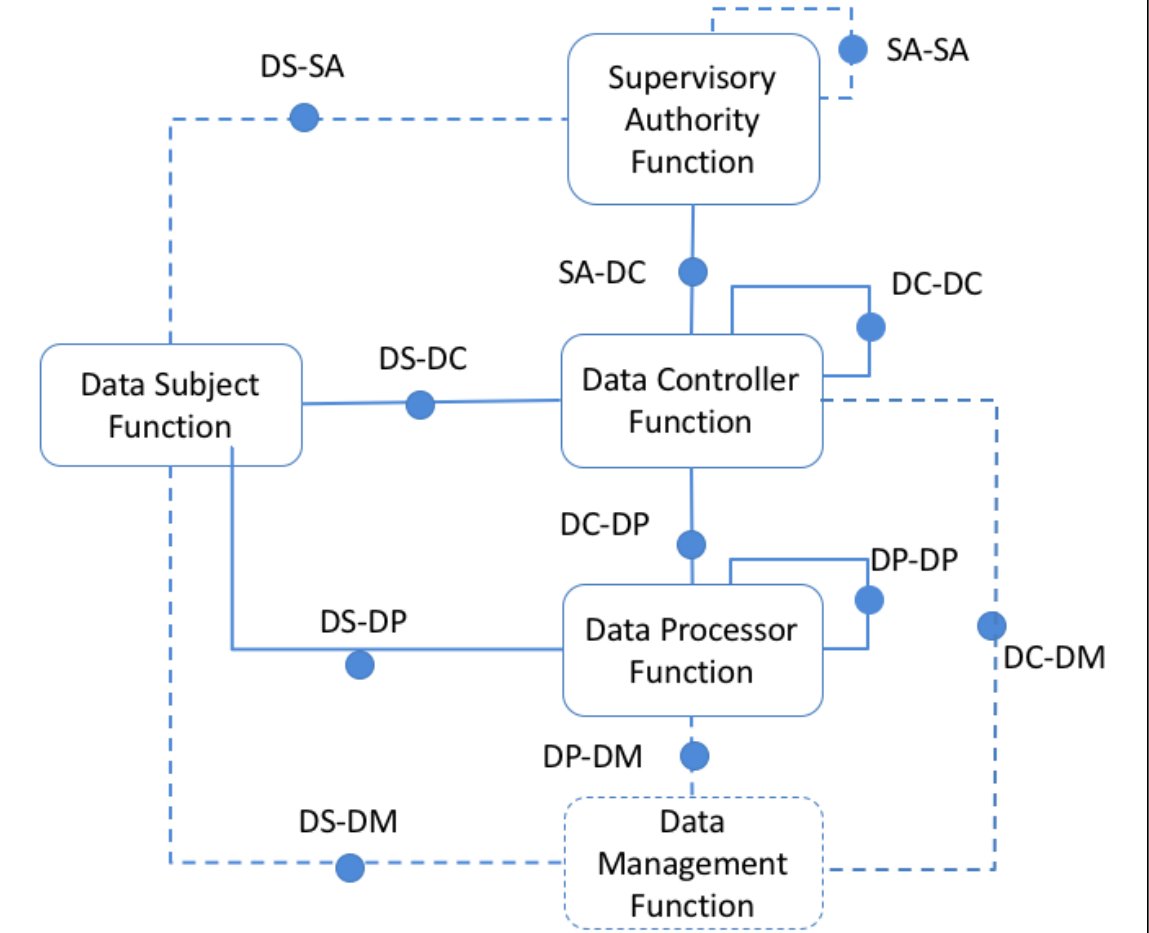
\includegraphics[width=0.75\linewidth]{img/interoperability-model.png}
    \caption{Model of information interoperability between entities based on requirements of GDPR \cite{pandit_exploration_2018}}
    \label{fig:info:interoperability-model}
\end{figure}
These points of interactions consist of information exchange between entities, are are guided by the requirements of compliance. For example, the interaction between data subject and data controller consists of the data subject providing personal data to the controller, while the controller is required to provide a copy of provided personal data for fulfilment of rights granted by the GDPR.

Requirements gathered from GDPR \cite{pandit_exploration_2018} provide the following categories of information flows between entities at points of interactions:
\begin{itemize}
    \item Provenance records: GDPR requires controllers and processors to maintain provenance records of processing activities carried out under their responsibility in order to maintain and demonstrate compliance to supervisory authorities. Provenance records are also required to be maintained to enable provision of rights to the data subject, and for information sharing between controllers and third parties.
    \item Data sharing agreements: A controller and processor are required to have specific data sharing agreements in place that specify the processing activities to be carried out by the processor. 
    \item Consent information: Consent information regarding how it was provided to the data subject and the given consent are required to be recorded for demonstrating compliance as well as for providing the right to withdraw consent. Consent information is also required to be passed on to other controllers or third parties (at the request of the data subject) if processing involves more than one party.
    \item Compliance documentation: Processors are required to provide suitable guarantees to controllers regarding measures that ensure compliance with the GDPR. This information needs to be shared between controllers and processors, as well as demonstrated to supervisory authorities in the due process of evaluating compliance.
    \item Use of certifications: GDPR provides seals and certifications to be used to denote a certain degree of compliance based on existence of measures and processes that adhere to GDPR requirements. The presence of such seals and certifications as well as their associated information needs to be exchanged between entities to demonstrate trust and guarantees, such as between processors and controllers, or controllers and data subjects.
\end{itemize}

% opportunities for commonality and interoperability
The model and analyses of information flows between entities provides the motivation for establishing interoperability in the representation of information to be exchanged. In particular, provenance records regarding activities associated with personal data and consent are associated with interactions between all entities - data subjects, controllers, processors, and supervisory authorities. Thus, provenance records are important to the documentation of compliance for all stakeholders. 

While provenance information is usually taken to refer to processing of personal data, information about other categories, namely - consent, data sharing agreements, compliance, and certifications - also can be represented using the same representation. This provides the advantage of using a single representation leading to a cohesive management of compliance information.

The use of process flows (ex-ante and ex-post) to represent information about processing activities is documented in the state of the art (see \autoref{chapter:sota}). In this, approaches have utilised existing standards such as PROV and BPMN. However, these approaches do not realise the potential to reuse the same representation towards other information categories.
For the scope of the thesis, the focus of representations is on categories of provenance records and consent information, while ensuring potential of reuse towards other categories through future extensions. This provides the broad motivation of developing an interoperable ontology for representing activities associated with personal data and consent - such that they can be utilised to also represent data sharing agreements and compliance agreements in the future.

\section{Compliance Questions}\label{sec:info:compliance-questions}
This section presents `compliance questions' whose answers provide information necessary for evaluating GDPR compliance. The questions are essential to the development of information representations within compliance management systems by providing requirements for the structuring of information and its validation. Within this thesis, they are used to guide the development of ontologies through creation of competency questions (see \autoref{sec:info:competency-questions}) and validation of information (see \autoref{sec:info:constraints}).

The questions were collected from authoritative sources such as data protection commissions, legal experts and agencies - that have published guidelines and resources to assist organisations with the process of establishing and maintaining GDPR compliance.
Amongst the provided resources are checklists or criteria to self-assess measure of GDPR compliance within an organisation. These were utilised as the primary source for compliance questions.
For the questions presented in this thesis, the following sources were used or referenced in addition to the text of GDPR:
\begin{itemize}
    \item Guidelines, clarifications, and discussions published by European Data Protection Board\footnote{\url{https://edpb.europa.eu/}} (EDPB)
    \item Guidelines, clarifications, and discussions published by Article 29 Working Party\footnote{\url{https://ec.europa.eu/newsroom/article29/news.cfm?item_type=1360}} and endorsed by EDPB
    \item Resources published Data Protection Commission\footnote{\url{https://dataprotection.ie/}} (Ireland) - with particular focus on document `GDPR guidance for SMEs'\footnote{\url{https://dataprotection.ie/en/guidance-landing/guidance-smes}}
    \item Resources published by Information Commissioners Office\footnote{\url{https://dataprotection.ie/}} (United Kingdom), with particular use of `Data protection self assessment for organisations'\footnote{\url{https://ico.org.uk/for-organisations/data-protection-self-assessment/}}
    \item Resources published by federated data protection offices in Germany, in particular the audit checklist published by Lower Saxony Data Protection Authority\footnote{\url{https://lfd.niedersachsen.de/download/146715/}} which was self-translated from German to English\footnote{\url{https://doi.org/10.5281/zenodo.3380469}}
    \item Resources regarding GDPR compliance published by professional institutions within legal compliance domain, specifically - Nymity\footnote{\url{https://info.nymity.com/gdpr-compliance-toolkit}} and IAPP\footnote{\url{https://iapp.org/resources/article/gdpr-genius/}}
    \item Executive and Court decisions regarding GDPR compliance, tracked using the online community service \url{https://www.enforcementtracker.com/} which also provides the article of GDPR relevant to the decision
\end{itemize}

The collected questions were rephrased and divided into smaller more granular questions towards establishment of information requirements and constraints. 
Each question was assigned an ID to enable referencing its use in competency questions presented in \autoref{sec:info:competency-questions} and further clarification of assumptions and constraints for validation presented in \autoref{sec:info:constraints}.
Where possible, each question was associated with specific clauses of the GDPR. 
% COMPLIANCCE QUESTIONS - CONTROLLERS
\begin{table}
\small
\centering
\caption{Compliance questions pertaining to records of processing activities to be kept by controllers}\label{table:info:compliance-controllers}
\begin{tabularx}{\textwidth}{|l|X|l|}
\hline
\textbf{ID} & \textbf{Compliance Question} & \textbf{GDPR ref.} \\ \hline

CMQ1 & How are the records of processing activities maintained? & R82,A30,A30-3 \\ \hline
CMQ2 & What is the name and identity of the controller(s) and their representatives/DPOs? & A30-1a \\ \hline
CMQ3 & What are the the purposes of processing? & A30-1b \\ \hline
CMQ4 & What are the categories of data subjects? & A30-1c \\ \hline
CMQ5 & What are the categories of personal data? & A30-1c \\ \hline
CMQ6 & Is data shared? &  \\ \hline
CMQ7 & If data is shared, what are the categories of recipients to whom the personal data is or will be disclosed? & A30-1d \\ \hline
CMQ8 & If data is shared, what are the identities of the recipients to whom the data is or will be disclosed? & A30-1d,A30-1e \\ \hline
CMQ9 & If data is shared, are the recipients to whom the data is or will be disclosed based in a Third Country or International Organisation? & A30-1e \\ \hline
CMQ10 & If data is shared, and the recipients are in a Third Country or International Organisation, what are the safeguards associated with data transfer? & A30-1e \\ \hline
CMQ11 & Is data stored? &  \\ \hline
CMQ12 & Where data is stored, its erasure is based on what critera: time limit or condition or event? &  \\ \hline
CMQ13 & Where data is stored, what are the time limits or conditions or events for erasure for different categories of data? & A30-1f \\ \hline
CMQ14 & What are the technical and organisational security measures w.r.t to the processing of personal data? & A30-1g \\ \hline
CMQ15 & Where data is shared, what are the purposes for sharing of personal data with the recipients? &  \\ \hline
\end{tabularx}
\end{table}
% COMPLIANCE QUESTIONS - PROCESSORS
\begin{table}
\small
\centering
\caption{Compliance questions pertaining to records of processing activities to be kept by processors}\label{table:info:compliance-processors}
\begin{tabularx}{\textwidth}{|l|X|l|}
\hline
\textbf{ID} & \textbf{Compliance Question} & \textbf{GDPR ref.} \\ \hline
CMQ16 & How are the records of processing activities maintained? & R82,A30,A30-3 \\ \hline
CMQ17 & What is the name and identity of the processor(s) and their representatives/DPOs? & A30-1a \\ \hline
CMQ18 & What is the name and identity of the controller(s) the processor is acting on behalf of? & A30-2a \\ \hline
CMQ19 & What are the the categories of processing carried out on behalf of the controller? & A30-2b \\ \hline
CMQ20 & If data is shared, what are the categories of recipients to whom the personal data is or will be disclosed? & A30-1d \\ \hline
CMQ21 & If data is shared, what are the identities of the recipients to whom the data is or will be disclosed? & A30-1d,A30-1e \\ \hline
CMQ22 & If data is shared, are the recipients to whom the data is or will be disclosed based in a Third Country or International Organisation? & A30-1e \\ \hline
CMQ23 & If data is shared, and the recipients are in a Third Country or International Organisation, what are the safeguards associated with data transfer? & A30-1e \\ \hline
CMQ24 & What are the technical and organisational security measures w.r.t to the processing of personal data? & A30-1g \\ \hline
CMQ25 & Where data is shared, what are the purposes for sharing of personal data with the recipients? &  \\ \hline
\end{tabularx}
\end{table}
% COMPLIANCE QUESTIONS - LEGAL BASIS
\begin{table}
\small
\centering
\caption{Compliance questions pertaining to legal basis of processing activities}\label{table:info:compliance-legal-basis}
\begin{tabularx}{\textwidth}{|l|X|l|}
\hline
\textbf{ID} & \textbf{Compliance Question} & \textbf{GDPR ref.} \\ \hline
CMQ26 & What is the legal basis for processing of data? \\ \hline
CMQ27 & What is the legal basis for the purpose for processing of data? \\ \hline
\end{tabularx}
\end{table}
% COMPLIANCE QUESTIONS - PERSONAL DATA
\begin{table}
\small
\centering
\caption{Compliance questions pertaining to personal data}\label{table:info:compliance-personal-data}
\begin{tabularx}{\textwidth}{|l|X|l|}
\hline
\textbf{ID} & \textbf{Compliance Question} & \textbf{GDPR ref.} \\ \hline
CMQ28 & What are the sources of personal data? \\ \hline
CMQ29 & What personal data are collected from the data subject? \\ \hline
CMQ30 & Where personal data are not collected from the data subject, what are their sources? \\ \hline
CMQ31 & Where data has been anonymised, what techniques were used for anonymisation? \\ \hline
CMQ32 & Can pseudo-anonymised data be de-anonymised by the organisation using information it already possesses or is available to it? \\ \hline
CMQ33 & What are the sources of personal data? \\ \hline
CMQ34 & What personal data are collected from the data subject? \\ \hline
\end{tabularx}
\end{table}
% COMPLIANCE QUESTIONS - GIVEN CONSENT
\begin{table}
\small
\centering
\caption{Compliance questions pertaining to given consent}\label{table:info:compliance-given-consent}
\begin{tabularx}{\textwidth}{|l|X|l|}
\hline
\textbf{ID} & \textbf{Compliance Question} & \textbf{GDPR ref.} \\ \hline
CMQ35 & Who is the Data Subject associated with consent? & A4-11 \\ \hline
CMQ36 & What are the Personal Data associated with consent? & R32,A4-11 \\ \hline
CMQ37 & What are the Purposes associated with consent? & R32,R42 \\ \hline
CMQ38 & What are the Data Processing associated with consent? & R32,A4-11 \\ \hline
CMQ39 & What is the current Status of consent? & A7-3 \\ \hline
CMQ40 & Who are the Data Controllers associated with consent? &  \\ \hline
CMQ41 & Who provided consent? & A7-2 \\ \hline
CMQ42 & Was consent provided by Delegation? & A8-c \\ \hline
CMQ43 & If consent was provided by Delegation, what was the role played by Delegate with respect to the Data Subject? &  \\ \hline
CMQ44 & If consent was provided by Delegation, how was the delegation executed? &  \\ \hline
CMQ45 & If consent was provided by Delegation, how was the delegate authenticated? & A8-2 \\ \hline
CMQ46 & Who was the consent given to? &  \\ \hline
CMQ47 & If consent was not given to the Data Controller, what is the relationship between the entity it was provided to and the Data Controller? &  \\ \hline
CMQ48 & How was the consent given/obtained? &  \\ \hline
CMQ49 & What artefacts were involved in the giving/obtaining of consent? &  \\ \hline
CMQ50 & What were the choices provided for consent? &  \\ \hline
CMQ51 & What was the statement or affirmative action indicating given consent? &  \\ \hline
CMQ52 & How was the right to withdraw consent communicated to the data subject? &  \\ \hline
CMQ53 & At what location was the consent given? &  \\ \hline
CMQ54 & What is the medium associated with consent? & R32,A7-2 \\ \hline
CMQ55 & What is the timestamp associated with the consent? &  \\ \hline
CMQ56 & What is the expiry of the consent? &  \\ \hline
CMQ57 & Is the purpose or processing associated with a third party? &  \\ \hline
CMQ58 & What is the role played by the third party in the purpose or processing? &  \\ \hline
CMQ59 & Does the processing of data involve storage of data? &  \\ \hline
CMQ60 & If personal data is being stored, what is the duration of storage for Personal Data? &  \\ \hline
CMQ61 & If personal data is being stored, what is the location of storage? &  \\ \hline
CMQ62 & Are processing associated with consent of automated nature? & R71,A9-2c,A22-2c \\ \hline
CMQ63 & Does the processing of data involve transfer to a Third Country or International Organisation? & R111,A49-1a \\ \hline
CMQ64 & If processing of data involves transfer to a Third Country or International Organisation, what is the identity of the Third Country or International Organisation? &  \\ \hline
CMQ65 & Do the personal data associated with consent belong to a special category? & R51,A8-2a \\ \hline
CMQ66 & How is personal data associated or linked to the data subject? &  \\ \hline
CMQ67 & Is the Data Subject of legal age to provide their own consent? & A8 \\ \hline
CMQ68 & What are the specific laws that determine the legal age to provide consent? & A8-1 \\ \hline
CMQ69 & Does the Data Subject have a specific relationship with the Data Controller? & R43 \\ \hline
\end{tabularx}
\end{table}
% COMPLIANCE QUESTIONS - CHANGE IN CONSENT STATE
\begin{table}
\small
\centering
\caption{Compliance questions pertaining to change in consent state}\label{table:info:compliance-change-consent}
\begin{tabularx}{\textwidth}{|l|X|l|}
\hline
\textbf{ID} & \textbf{Compliance Question} & \textbf{GDPR ref.} \\ \hline

CMQ70 & Who is the Data Subject associated with consent? & A4-11 \\ \hline
CMQ71 & What are the Personal Data associated with consent? & R32,A4-11 \\ \hline
CMQ72 & What are the Purposes associated with consent? & R32,R42 \\ \hline
CMQ73 & What are the Data Processing associated with consent? & R32,A4-11 \\ \hline
CMQ74 & What is the current state/status of consent? & A7-3 \\ \hline
CMQ75 & Who are the Data Controllers associated with consent? &  \\ \hline
CMQ76 & Who changed the state/status of consent? &  \\ \hline
CMQ77 & Was consent changed by Delegation? &  \\ \hline
CMQ78 & If consent was changed by Delegation, what was the role played by Delegate with respect to the Data Subject? &  \\ \hline
CMQ79 & If consent was changed by Delegation, how was the delegation executed? &  \\ \hline
CMQ80 & If consent was changed by Delegation, how was the delegate authenticated? & A8-2 \\ \hline
CMQ81 & How was the consent state/status changed? &  \\ \hline
CMQ82 & What artefacts were involved in the change in state/status of consent? &  \\ \hline
CMQ83 & If change in consent was done by the Data Subject, what was the statement or affirmative action indicating change to their consent? &  \\ \hline
CMQ84 & At what location was the consent changed? &  \\ \hline
CMQ85 & What is the medium associated with change in consent? & R32,A7-2 \\ \hline
CMQ86 & What is the timestamp associated with the consent? &  \\ \hline
CMQ87 & If the current state/status of consent is valid for processing, what is the expiry of the consent? &  \\ \hline
\end{tabularx}
\end{table}
% COMPLIANCE QUESTIONS - RIGHT TO BE INFORMED
\begin{table}
\small
\centering
\caption{Compliance questions pertaining to provision of right to be informed}\label{table:info:compliance-right-informed}
\begin{tabularx}{\textwidth}{|l|X|}
\hline
\textbf{ID} & \textbf{Compliance Question} \\ \hline
CMQ88 & How was information relevant for the right to be informed provided to the data subjects? \\ \hline
CMQ89 & When was the information relevant to right to be informed was provided to the data subject? \\ \hline
CMQ90 & Was the name and contact details of the controller’s representative provided to the data subject under the right to be informed? \\ \hline
CMQ91 & Was the name and contact details of the DPO provided to the data subject under the right to be informed? \\ \hline
CMQ92 & Was the purposes for processing provided to the data subject under the right to be informed? \\ \hline
CMQ93 & Was the legal basis for processing provided to the data subject under the right to be informed? \\ \hline
CMQ94 & Where the legal basis for processing was legitimate interest, was this communicated to the data subject under the right to be informed? \\ \hline
CMQ95 & If personal data is not obtained from the data subject, were the categories of personal data obtained communicated to the data subject under the right to be informed? \\ \hline
CMQ96 & If personal data is not obtained from the data subject, were the sources of data communicated to the data subject under the right to be informed? \\ \hline
CMQ97 & Where personal data is shared, were the recipients or categories of recipients communicated to the data subject under the right to be informed? \\ \hline
CMQ98 & If personal data is transferred to a third country or international organisation, were the identity of the third country or international organisation communicated to the data subject under the right to be informed? \\ \hline
CMQ99 & Where personal data is stored, were the retention period communicated to the data subject under the right to be informed? \\ \hline
CMQ100 & Were the rights available communicated to the data subject under the right to be informed? \\ \hline
CMQ101 & If the data subject provided consent, was the right to withdraw consent provided under the right to be informed? \\ \hline
CMQ102 & Was the right to lodge a complaint with a supervisory authority provided to the data subject under the right to be informed? \\ \hline
CMQ103 & Where personal data needs to be provided under statutory or contractual obligation, was this communicated to the data subject under the right to be informed? \\ \hline
CMQ104 & Where personal data needs to be provided under statutory or contractual obligation, and if this data needs to be obtained from the data subject, was this communicated to the data subject under the right to be informed? \\ \hline
CMQ105 & Where automated-decision making, including profiling is used, was this communicated to the data subject under the right to be informed? \\ \hline
\end{tabularx}
\end{table}
% COMPLIANCE QUESTIONS - DATA BREACH
\begin{table}
\small
\centering
\caption{Compliance questions pertaining to reporting of data breach by controllers}\label{table:info:compliance-data-breach}
\begin{tabularx}{\textwidth}{|l|X|l|}
\hline
\textbf{ID} & \textbf{Compliance Question} & \textbf{GDPR ref.} \\ \hline
CMQ106 & When did the data breach occur? &  \\ \hline
CMQ107 & When did the controller become aware of the data breach? & R85,R33-1 \\ \hline
CMQ108 & Was the data breach notified to the supervisory authority? &  \\ \hline
CMQ109 & When was the notification of data breach provided to the supervisory authority? & R85 \\ \hline
CMQ110 & How was the notification of data breach provided to the supervisory authority? & R85,R33-1 \\ \hline
CMQ111 & Is the data breach likely to result in a high risk to the rights and freedoms of the natural person whose data is associated with it? & R86,A33-1,A34-1 \\ \hline
CMQ112 & Who are the data subjects whose personal data are associated with the data breach? &  \\ \hline
CMQ113 & Was the data breach notified to the data subjects? &  \\ \hline
CMQ114 & When was the notification of data breach provided to the data subjects? &  \\ \hline
CMQ115 & How was the notification of data breach provided to the data subjects? & R85,R33-1 \\ \hline
CMQ116 & How did the notification of data breach to the data subject provide information about the data breach? & R86,A34-2 \\ \hline
CMQ117 & How did the notification of data breach to the data subject provide information about mitigating potential effects? & R86,A34-2 \\ \hline
CMQ118 & What data was involved in the data breach? &  \\ \hline
CMQ119 & What technical measures were in place for the protection of data involved in the data breach? & R88 \\ \hline
CMQ120 & What steps were taken to prevent or mitigate the effects of the data breach? &  \\ \hline
\end{tabularx}
\end{table}

\section{Constraints \& Assumptions for Validation}\label{sec:info:constraints}

\section{Competency Questions}\label{sec:info:competency-questions}

